% Drawing 80/02-3 -- folder 80, batch 02, archive page 24 (PDF page 25).
% Transcription: à droite, un dessin : six droites, les côtés d'un triangle et trois droites issues de ses sommets concourant en un point intérieur ; quatre points triples marqués
% Kind: triangle with three concurrent cevians. Method 2 (schematic redraw from the facsimile). Status: ok.
% Notes: Six lines: the sides of a triangle and three lines from its vertices meeting at an interior point; four triple points marked heavy (the three vertices and the interior point). The complete quadrilateral with its diagonals in the middle of the page belongs to the text ("arrangement d'un quadrilatère et de ses diagonales") and has no mark; it is not drawn.
% Coordinates: 1 unit = 1 mm = 1/100 of the crop width (bbox in page fractions: [0.68, 0.3, 0.86, 0.38]).
% Redrawn by Claude (claude-opus-5-5), issue #73, 2026-11-07; not checked by a human; not compiled (no TeX in the session).
% Revised 2026-11-07 after Michel's check: the cevians now meet exactly at the interior point and the sides at the vertices (four triple points).
% Rights: reproduces part of the work -- behind RENDER_TRANSCRIPTS, never published by itself.
\documentclass[tikz,border=3pt]{standalone}
\usepackage{amsmath,amssymb}
\usetikzlibrary{patterns,arrows.meta}
\tikzset{pencil/.style={black!45}, struck/.style={black!35}, mark/.style={circle,draw,inner sep=1.3pt}, pt/.style={circle,fill,inner sep=0.9pt}, opt/.style={circle,draw,fill=white,inner sep=1.1pt}}
\begin{document}
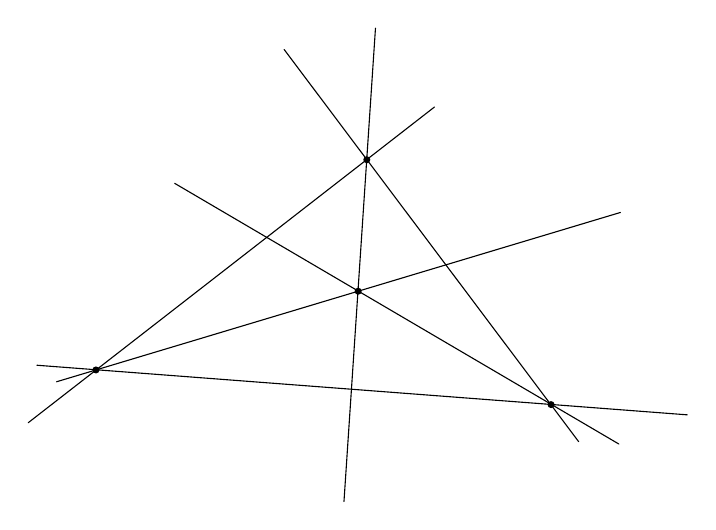
\begin{tikzpicture}[x=1mm,y=1mm,line cap=round,line join=round,font=\scriptsize]
\draw (0.3,-43.8) -- (82.9,-50.1);
\draw (-0.8,-51.1) -- (50.8,-11.0);
\draw (31.7,-3.7) -- (69.1,-53.5);
\draw (43.3,-1.0) -- (39.3,-61.1);
\draw (74.2,-53.8) -- (17.8,-20.7);
\draw (2.8,-45.9) -- (74.4,-24.4);
\node[pt] at (42.2,-17.7) {};
\node[pt] at (41.1,-34.4) {};
\node[pt] at (7.8,-44.4) {};
\node[pt] at (65.6,-48.8) {};
\end{tikzpicture}
\end{document}
